%%%%%%%%%%%%%%%%%%%%%%%%%%%%%%%%%%%%%%%%%
% University/School Laboratory Report
% This is for code review purposes only
% 
% Authors:
% Szymon Zinkowicz
%
% License:
% MIT
%
%%%%%%%%%%%%%%%%%%%%%%%%%%%%%%%%%%%%%%%%%

\documentclass[
	report, % Paper size, specify a4paper (A4) or letterpaper (US letter)
	11pt, % Default font size, specify 10pt, 11pt or 12pt
]{CSUniSchoolLabReport}

\usepackage[table, dvipsnames]{xcolor}
\usepackage{hyperref}
\usepackage{graphicx}
\usepackage{subcaption} % To have subfigures available
\usepackage{caption} % To have caption justification
\usepackage[export]{adjustbox}
\usepackage{lipsum} % for mock text
\usepackage{fancyhdr}
\usepackage{csvsimple} % for reading csv
\usepackage{float} % for H in figures
\usepackage{siunitx} % for SI units and rounding
\usepackage{pgfplotstable}  % For handling table imports and formatting
\usepackage{booktabs}       % For professional table formatting
\usepackage{pgffor}   % For looping constructs
\usepackage{array,multirow,makecell}
\usepackage{pdflscape}
\usepackage{forloop}  % For creating loop-like behavior
\usepackage{geometry} % For setting the margins
\usepackage{listings}
\usepackage{changepage}
\newcounter{ct}
\newcommand{\addimage}[1]{%
    \begin{minipage}{0.48\textwidth}
        \centering
        \includegraphics[width=\linewidth]{#1}
    \end{minipage}%
}

\newcolumntype{R}[1]{>{\raggedleft\arraybackslash }b{#1}}
\newcolumntype{L}[1]{>{\raggedright\arraybackslash }b{#1}}
\newcolumntype{C}[1]{>{\centering\arraybackslash }b{#1}}

\sisetup{
  round-mode = places, % Rounds numbers
  round-precision = 4, % to 4 decimal places
}
\addbibresource{sample.bib} % Bibliography file (located in the same folder as the template)
% \lstset { %
%     language=C++,
%     backgroundcolor=\color{black!5}, % set backgroundcolor
%     basicstyle=\footnotesize,% basic font setting
% }
\hypersetup{
	colorlinks=true,
	linktoc=all,
	linkcolor=blue,
}

\pagestyle{fancy}
\fancyhf{}
\fancyhead[L]{Mandelbrot Program Performance Analysis}
\fancyhead[R]{December 28, 2024}
\fancyfoot[C]{\thepage}
\renewcommand{\headrulewidth}{2pt}
\renewcommand{\footrulewidth}{1pt}
\renewcommand{\sectionmark}[1]{\markboth{\thesection. #1}{}}
\fancyhead[L]{%
  \begin{tabular}{@{}l@{}}
  \leftmark\\
  \rightmark
  \end{tabular}%
}
\setlength{\headheight}{24pt}
\definecolor{codegreen}{rgb}{0,0.6,0}
\definecolor{codegray}{rgb}{0.5,0.5,0.5}
\definecolor{codepurple}{rgb}{0.58,0,0.82}
\definecolor{backcolour}{rgb}{0.95,0.95,0.92}

\lstdefinestyle{cppstyle}{
    backgroundcolor=\color{backcolour},   
    commentstyle=\color{codegreen},
    keywordstyle=\color{magenta},
    numberstyle=\tiny\color{codegray},
    stringstyle=\color{codepurple},
    basicstyle=\ttfamily\footnotesize,
    breakatwhitespace=false,         
    breaklines=true,                 
    captionpos=b,                    
    keepspaces=true,                 
    numbers=left,                    
    numbersep=5pt,                  
    showspaces=false,                
    showstringspaces=false,
    showtabs=false,                  
    tabsize=2
}
\lstset{style=cppstyle}
%----------------------------------------------------------------------------------------
%	Functions ;>
%----------------------------------------------------------------------------------------

\newcommand{\getcols}[1]{%
    \ifx\relax#1\relax\else
        \csvcoli[\numexpr#1-1]%
        \getcols
    \fi
}

\newcommand{\csvtablecols}[5]{%
    \begin{table}[H]
        \centering
        \rowcolors{3}{white}{lightgray}
        \csvreader[
            tabular=|*{3}{c|},
            table head=\hline \rowcolor{SeaGreen} #3 \\\hline,
            late after line=\\\hline,
            before reading={\rowcolors{3}{white}{lightgray}}
        ]{#1}%
        {#5}%
        {\iterations & \resolution & \execTime}
        \caption{#2}
    \end{table}
}

%----------------------------------------------------------------------------------------
%	REPORT INFORMATION
%----------------------------------------------------------------------------------------



\begin{document}

\title{HIGH PERFORMANCE COMPUTING \\
	\large Final Project Report \\
	Mandelbrot Set
	Computation} % Title
\author{Szymon \textsc{Zinkowicz} \\ Matricola number: 5181814} % Author name(s)
\date{\today} % Date of the report

\maketitle % Insert the title, author, and date using the information specified above
\thispagestyle{empty}

\begin{center}
	\vspace{\fill}
	University of \textsc{Genova} \\
	\begin{tabular}{l r}
		Instructor: & Professor \textsc{Daniele D'agostino}
	\end{tabular}
\end{center}
\pagebreak



%----------------------------------------------------------------------------------------
%	Abstract
%----------------------------------------------------------------------------------------
\begin{abstract}
	\thispagestyle{empty}The computation of the Mandelbrot Set, a quintessential example of complex fractal geometry, serves as a benchmark for evaluating the performance and scalability of High-Performance Computing (HPC) systems. This report presents a comprehensive analysis of Mandelbrot Set computations executed across various computational environments and parallelization paradigms.

	We employed C and C++ programming languages to implement the algorithm, utilizing different compiler optimizations including G++ 13.3.0 and AOCC-compiler 5.0.0 on a local setup equipped with an AMD processor. To explore parallel processing capabilities, the study integrates OpenMP for shared-memory parallelism and CUDA leveraging an RTX 2070 GPU on a laptop platform.

	Furthermore, distributed computing was investigated using the Message Passing Interface (MPI) on a cluster of machines, assessing the scalability and efficiency of the implementation in a multi-node environment. Benchmarking results indicate significant performance enhancements through parallelization, with CUDA and MPI-based approaches demonstrating substantial reductions in computation time compared to sequential executions.


	The comparative analysis underscores the advantages and trade-offs of each setup, providing critical insights for optimizing fractal computations in diverse HPC architectures. This work contributes to the broader understanding of parallel computing strategies, offering practical guidelines for leveraging modern hardware and software tools to accelerate complex mathematical computations.
\end{abstract}
\pagebreak

%----------------------------------------------------------------------------------------
%	Table of Contents
%----------------------------------------------------------------------------------------
\tableofcontents % Insert the table of contents
\thispagestyle{empty}
\pagebreak

\section{Introduction}

The Mandelbrot Set is one of the most renowned examples of complex fractal geometry, serving both as a subject of mathematical intrigue and as a benchmark for computational performance in High-Performance Computing (HPC). Named after the mathematician Benoît B. Mandelbrot, the set exemplifies the intricate boundary structures that emerge from simple iterative processes.

Mathematically, the Mandelbrot Set is defined in the complex plane and consists of all complex numbers \( c \) for which the sequence \( \{ z_n \} \) remains bounded when iteratively applying the function:

\begin{equation}
	z_{n+1} = z_n^2 + c,
\end{equation}

where \( z_0 = 0 \). Here, both \( z \) and \( c \) are complex numbers, expressed as \( z = x + yi \) and \( c = a + bi \), with \( x, y, a, b \in \mathbb{R} \) and \( i \) being the imaginary unit.

The iterative process starts with \( z_0 = 0 \) and generates successive terms by repeatedly applying the quadratic polynomial. The key question in the study of the Mandelbrot Set is determining whether the sequence \( \{ z_n \} \) remains bounded as \( n \) approaches infinity. If the magnitude of \( z_n \) does not tend to infinity, the complex number \( c \) is said to belong to the Mandelbrot Set.

\begin{figure}[h]
	\centering
	\captionsetup{justification=centering, width=.8\linewidth}
	
\includegraphics[width=0.6\textwidth]{./img/mandelbrot-set-google.jpg}
	\caption{Visualization of the Mandelbrot Set in the complex plane. Points within the set are typically colored black, while points outside the set are colored based on the rate at which the sequence \( \{ z_n \} \) diverges.}
	\label{fig:mandelbrot}
\end{figure}

\noindent Figure~\ref{fig:mandelbrot} illustrates a common representation of the Mandelbrot Set. Each point \( c = a + bi \) in the complex plane is tested for membership in the set by iterating the aforementioned equation. The boundary of the Mandelbrot Set exhibits an infinitely complex structure, characterized by self-similarity and intricate patterns at every scale, which are hallmark features of fractals.

From a computational perspective, generating high-resolution images of the Mandelbrot Set is computationally intensive, especially when exploring regions near the boundary where the behavior of the sequence \( \{ z_n \} \) becomes highly sensitive to initial conditions. This sensitivity necessitates a significant number of iterations to accurately determine the boundedness of the sequence, making the Mandelbrot Set an excellent candidate for performance benchmarking in HPC environments.

Furthermore, each point \( c \) of the Mandelbrot can be evaluated independently — makes it well-suited for various parallel computing paradigms, including OpenMP, MPI, and GPU architectures. This report delves into the implementation and performance analysis of Mandelbrot Set computations across different HPC setups, highlighting the efficiencies and challenges associated with each parallelization strategy.
\pagebreak

\subsection{Mathematical Foundations}

To formalize the criteria for membership in the Mandelbrot Set, consider the iterative function:

\begin{equation}
	f_c(z) = z^2 + c,
\end{equation}

where \( c \in \mathbb{C} \) is a complex parameter. Starting with \( z_0 = 0 \), the sequence \( \{ z_n \} \) is generated by:

\begin{equation}
	z_{n+1} = f_c(z_n) = z_n^2 + c.
\end{equation}


In practice, the sequence is iterated up to a maximum number of iterations \( N_{\text{max}} \). If \( |z_n| \) exceeds 2 before reaching \( N_{\text{max}} \), the point \( c \) is considered to escape to infinity and is thus not part of the Mandelbrot Set. The choice of \( N_{\text{max}} \) balances computational load with the accuracy of the boundary determination.

The boundary of the Mandelbrot Set is where the most computational effort is concentrated, as points near the boundary require a higher number of iterations to resolve their membership status accurately. This characteristic makes the Mandelbrot Set a challenging and insightful problem for assessing the capabilities of various HPC systems and parallel computing techniques.
\pagebreak

\subsection{Hardware and Software Setup} \label{ssec:Hardware and Software Setup}

This section outlines the hardware configuration used for the MandelBrot Set compuations.

\begin{table}[!htb]
	\captionsetup{justification=centering, width=.8\linewidth}
	\centering
	\begin{tabular}{ll}
		\hline
		\textbf{Attribute}        & \textbf{Specification}                    \\
		\hline
		\textbf{Model}            & AMD Ryzen 7 4800H                         \\
		\textbf{Architecture}     & Zen 2 AMD64 Family 23 Model 96 Stepping 1 \\
		\textbf{Instruction set}  & x86                                       \\
		\textbf{Cores}            & 8                                         \\
		\textbf{Threads}          & 16                                        \\
		\textbf{Base Clock Speed} & 2.9 GHz                                   \\
		\textbf{Max Clock Speed}  & 4.2 GHz                                   \\
		\textbf{L1 Cache}         & 64 KB per core                            \\
		\textbf{L2 Cache}         & 512 KB per core                           \\
		\textbf{L3 Cache}         & 8 MB                                      \\
		\hline
	\end{tabular}
	\caption{CPU Specifications}
	\label{tab:cpu_specs}
\end{table}

\begin{table}[!htb]
	\captionsetup{justification=centering, width=.8\linewidth}
	\centering
	\begin{tabular}{ll}
		\hline
		\textbf{Attribute}         & \textbf{Specification}  \\
		\hline
		\textbf{Model}             & NVIDIA GeForce RTX 2060 \\
		\textbf{CUDA Cores}        & 1920                    \\
		\textbf{Memory}            & 6 GB GDDR6              \\
		\textbf{Memory Bus Width}  & 192-bit                 \\
		\textbf{Max Clock Rate}    & 1.20 GHz                \\
		\textbf{Memory Clock Rate} & 5.501 GHz               \\
		\hline
	\end{tabular}
	\caption{GPU Specifications}
	\label{tab:gpu_specs}
\end{table}

Following compilers were used for the project:
\begin{itemize}
	\item GCC/G++ 13.3.0 (May 21, 2024)
	\item AOCC-compiler 5.0.0 (Clang based 17.0.6, September 24 2024)
	\item NVIDIA CUDA 12.4.131
\end{itemize}

\section{Methodology}

This section delineates the methodological approach undertaken to evaluate the performance of Mandelbrot Set computations across various HPC configurations. The primary objective was to benchmark the execution time and scalability of the Mandelbrot algorithm under different computational paradigms and optimization strategies. The methodology encompasses the following key components:

\subsection{Experimental Setup}

The experiments were conducted on a local machine equipped with an AMD Ryzen 7 4800H CPU and an NVIDIA GeForce RTX 2060 GPU. The system specifications are detailed in Subsection~\ref{ssec:Hardware and Software Setup}. The programming languages utilized were C and C++, leveraging compiler optimizations and parallelization techniques to enhance computational efficiency.

\subsection{Benchmark Parameters}

Two primary parameters were varied to assess their impact on performance:

\begin{itemize}
	\item \textbf{Iterations:} The number of iterations for the Mandelbrot computation was set to 1000, 2000, and 4000. Increasing the number of iterations enhances the accuracy of the fractal boundary but also escalates computational demand.
	\item \textbf{Resolution:} The resolution of the Mandelbrot image was varied among 1000, 2000, 4000, and 8000 pixels. Higher resolutions provide more detailed visualizations at the cost of increased memory usage and processing time.
\end{itemize}

\subsection{Compiler Optimizations}

To optimize the performance of the Mandelbrot computations, two compilers were employed: G++ (version 13.3.0) and AOCC (version 5.0.0). Various compiler flags were utilized to enable different optimization levels and architecture-specific enhancements. The flags used for each compiler are summarized in Table~\ref{tab:compiler_flags}.

\begin{table}[H]
	\centering
	\begin{tabular}{lp{9cm}}
		\hline
		\textbf{Compiler}  & \textbf{Flags}                                \\
		\hline
		\textbf{G++}       & \texttt{-Ofast -march=znver2 -mtune=znver2}   \\
		\hline
		\textbf{AOCC}      & \texttt{-Ofast -march=znver2 -mtune=znver2}   \\
		                   & \texttt{-ffp-contract=fast -zopt}             \\
		                   & \texttt{-mllvm -enable-strided-vectorization} \\
		                   & \texttt{-mllvm -global-vectorize-slp=true}    \\
		\hline
		\textbf{CUDA}      & \texttt{-tp=znver2 -fast -O4}                 \\
		\texttt{(nvc++)}   & \texttt{-Xcompiler -Wall}                     \\
		\hline
		\textbf{MPI}       & \texttt{-std=c++17 -fopenmp -Ofast}           \\
		\texttt{(mpiicpc)} & \texttt{-march=native -xHost -Wall}           \\
		\hline
	\end{tabular}
	\caption{Compiler Flags Used for Optimization}
	\label{tab:compiler_flags}
\end{table}

These flags were chosen to maximize performance by enabling aggressive optimization levels, targeting specific CPU architectures (e.g., \texttt{znver2} for AMD Zen 2).

\subsection{Implementation Configurations}

The Mandelbrot Set computation was implemented and benchmarked under various configurations, each leveraging different parallelization techniques and computational resources. The configurations are outlined as follows:

\subsubsection{Sequential Execution}

Initial benchmarks were conducted using a sequential implementation of the Mandelbrot algorithm. Both G++ and AOCC compilers were used to compile the sequential code with varying optimization levels. This baseline facilitates the comparison of performance improvements achieved through parallelization.

\subsubsection{OpenMP Parallelization}

To exploit shared-memory parallelism, OpenMP was integrated into the Mandelbrot implementation. The parallelization was tested with different numbers of threads (2, 4, 8, 16) and scheduling strategies (Dynamic, Static, Guided, Runtime). The Makefile targets \texttt{amd-openmp} and \texttt{gpp-openmp} were used to compile the OpenMP-enabled executables. The compiler flags \texttt{-fopenmp} and \texttt{-DSCHEDULE\_<SCHEDULER>=1} were employed to enable OpenMP support and define the scheduling strategy, respectively.

\subsubsection{MPI Distributed Computing}

For distributed-memory parallelism, the Message Passing Interface (MPI) was utilized. The MPI implementation was compiled using \texttt{mpiicpc} with appropriate optimization flags. Benchmarks were conducted on a cluster of machines, scaling the number of MPI processes from 16 up to 3072 nodes. The Makefile targets \texttt{compile-mpi} and \texttt{run-mpi} facilitated the compilation and execution of the MPI-based Mandelbrot program. The MPI benchmarks evaluated both strong and weak scaling performance by varying the number of nodes and processes per machine.

\subsubsection{CUDA GPU Acceleration}

To leverage GPU acceleration, a CUDA implementation of the Mandelbrot algorithm was developed and compiled using \texttt{nvc++}. The CUDA configuration targeted the NVIDIA GeForce RTX 2060 GPU, utilizing its 1920 CUDA cores for parallel computation. The Makefile targets \texttt{cuda} and \texttt{run-cuda} were used to compile and execute the CUDA-based Mandelbrot program. Different thread block sizes (2, 4, 8, 16, 32) were tested to optimize GPU utilization.

\subsection{Compilation and Execution}

The Makefile provided orchestrates the compilation and execution of the various Mandelbrot implementations. Key aspects of the Makefile include:

\begin{itemize}
	\item \textbf{Directory Structure:} Separate directories for binaries (\texttt{./bin/}), output files (\texttt{./out/}), and source code (\texttt{./src/}) ensure organized management of build artifacts.
	\item \textbf{Compiler Definitions:} Variables such as \texttt{CC}, \texttt{G++}, \texttt{NVC}, and \texttt{MPICC} are defined for ease of use across different compilation targets.
	\item \textbf{Optimization Flags:} Compiler flags are meticulously defined to tailor the build process for each computational paradigm, enabling optimizations specific to the hardware and parallelization strategy.
	\item \textbf{Benchmark Targets:} Targets like \texttt{run-all}, \texttt{run-openmp}, \texttt{run-mpi}, and \texttt{run-cuda} automate the execution of benchmarks across all configurations, iterating over the defined ranges of iterations and resolutions.
\end{itemize}

\subsection{Benchmarking Procedure}

The benchmarking process followed a systematic approach:

\begin{enumerate}
	\item \textbf{Compilation:} All implementations (sequential, OpenMP, MPI, CUDA) were compiled using their respective compiler targets in the Makefile. Optimization flags were applied to enhance performance.
	\item \textbf{Execution:} Each compiled executable was run with varying iterations and resolutions. For parallel implementations, additional parameters such as the number of threads or MPI processes were varied.
	\item \textbf{Data Collection:} Execution times and resource utilizations were recorded for each configuration. Output files generated by the programs served as logs for performance analysis.
	\item \textbf{Scalability Analysis:} The impact of increasing computational resources (e.g., more threads, higher resolutions) on performance was analyzed to assess scalability.
\end{enumerate}

\subsection{Code Benchmarking}

The core Mandelbrot computation was encapsulated within separate source files tailored to each parallelization strategy. Below is a representative snippet of the sequential Mandelbrot implementation, which served as the foundation for all parallel variants.

\begin{lstlisting}[language=C++, caption={Sequential Mandelbrot Implementation}, label={lst:mandelbrot_seq}]
int row = 0, col = 0;
for (int pos = 0; pos < HEIGHT * WIDTH; pos++)
{
	image[pos] = 0;
	row = pos / WIDTH;
	col = pos % WIDTH;
	const complex<double> c(
		col * STEP + MandelbrotSet::MIN_X,
		row * STEP + MandelbrotSet::MIN_Y
	);

	// z = z^2 + c
	complex<double> z(0, 0);
	for (int i = 1; i <= iterations; i++)
	{
		z = z * z + c;
		// If it is convergent
		if (abs(z) >= 2)
		{
			image[pos] = i;
			break;
		}
	}
}
\end{lstlisting}

\noindent Similar implementations were developed for OpenMP, MPI, and CUDA, each incorporating the necessary parallel constructs and optimizations to leverage the underlying hardware effectively. The benchmarking focused on measuring the execution time and evaluating the efficiency gains achieved through parallelization.

\subsection{Optimization Flags Justification}

The selection of compiler flags was pivotal in maximizing the performance of the Mandelbrot computations. The flags were chosen based on their ability to:

\begin{itemize}
	\item \textbf{Enable Aggressive Optimization:} Flags like \texttt{-Ofast} and \texttt{-O4} enable high levels of optimization, including vectorization and loop unrolling, which are essential for computationally intensive tasks.
	\item \textbf{Target Specific Architectures:} Flags such as \texttt{-march=znver2} and \texttt{-mtune=znver2} ensure that the generated code is optimized for the AMD Zen 2 architecture, leveraging its specific instruction sets and capabilities.
	\item \textbf{Facilitate Parallelization:} Flags like \texttt{-fopenmp} enable OpenMP support, while \texttt{-tp=znver2} in CUDA compilation targets the specific GPU architecture for optimal performance.
\end{itemize}

The deliberate selection and combination of these flags were instrumental in harnessing the full potential of the underlying hardware, ensuring that each implementation variant was as performant as possible.

\subsection{Data Analysis}

Post-execution, the collected benchmark data were analyzed to evaluate the performance metrics of each configuration. Key performance indicators included:

\begin{itemize}
	\item \textbf{Execution Time:} The total time taken to complete the Mandelbrot computation for each configuration.
	\item \textbf{Scalability:} The ability of the implementation to effectively utilize additional computational resources (e.g., more threads or MPI processes) to reduce execution time.
	\item \textbf{Speedup:} The ratio of performance gains to the resources utilized, indicating the effectiveness of the parallelization strategy.
\end{itemize}

Graphs and tables were generated to visualize the performance trends, highlighting the strengths and limitations of each computational approach. This analysis provided insights into the optimal configurations for Mandelbrot Set computations on the given HPC setup.

\subsection{Reproducibility and Code Availability}

To ensure reproducibility of the results, all source code, Makefile configurations, and benchmark scripts are maintained in a version-controlled repository. Interested readers and researchers can access the codebase to replicate the experiments or adapt the implementations for related studies.

\section{Benchmarks}

This section presents the benchmarking results of the Mandelbrot Set computations across various configurations and compiler optimizations. The performance metrics include execution times for different iterations and resolutions, as well as a comparative analysis between G++ and AOCC compilers.

\subsection{Sequential Execution}

\begin{table}[H]
	\centering
	\captionsetup{justification=centering, width=.8\linewidth}
	\rowcolors{2}{gray!25}{white}
	\begin{tabular}{rrrrr}
\toprule
Resolution & Iterations & G++ Time (s) & AOCC Time (s) & Speedup \\
\midrule
1000 & 1000 & 5.132 & 3.697 & 1.388 \\
2000 & 1000 & 20.808 & 14.549 & 1.430 \\
4000 & 1000 & 83.057 & 57.558 & 1.443 \\
8000 & 1000 & 333.786 & 228.167 & 1.463 \\
1000 & 2000 & 10.142 & 7.185 & 1.412 \\
2000 & 2000 & 41.170 & 28.259 & 1.457 \\
4000 & 2000 & 163.894 & 113.408 & 1.445 \\
8000 & 2000 & 652.484 & 451.177 & 1.446 \\
1000 & 4000 & 20.160 & 14.300 & 1.410 \\
2000 & 4000 & 81.168 & 56.410 & 1.439 \\
4000 & 4000 & 324.615 & 226.171 & 1.435 \\
8000 & 4000 & 1269.810 & 896.245 & 1.417 \\
\bottomrule
\end{tabular}

	\caption{Comparison of execution times for G++/AOCC-compiled sequential Mandelbrot computations across different iterations and resolutions.}
	\label{tab:mandelbrot_gcc_vs_aocc_comparison}
	\rowcolors{1}{}{ }
\end{table}

\begin{figure}[H]
	\captionsetup{justification=centering, width=.8\linewidth}
	\centering
	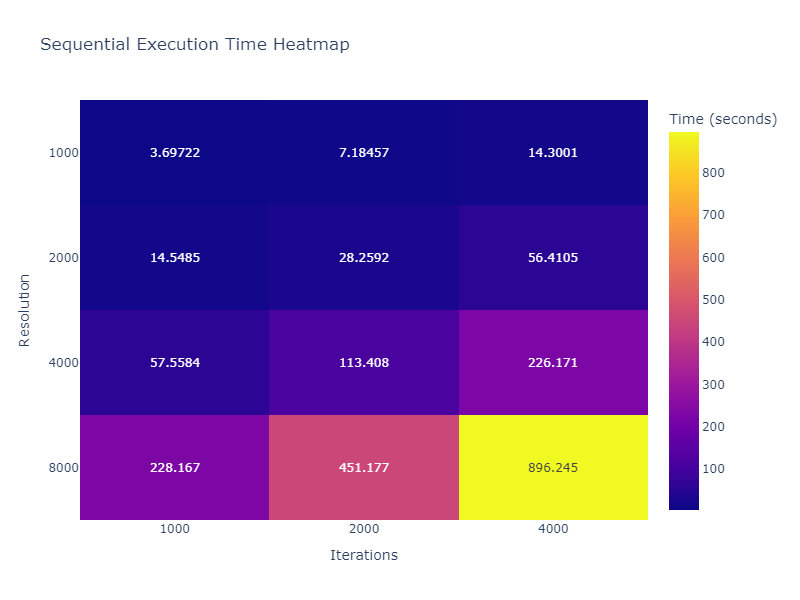
\includegraphics[width=\textwidth]{./img/mandelbrot_aocc_seq_heatmap.png}
	\caption{Heatmap of Execution Times for AOCC Sequential Mandelbrot Computations with varying iterations and resolutions.}
	\label{fig:mandelbrot_aocc_seq_heatmap}
\end{figure}

\subsubsection{G++ vs AOCC Performance Comparison}

\begin{figure}[H]
	\captionsetup{justification=centering, width=.8\linewidth}
	\centering
	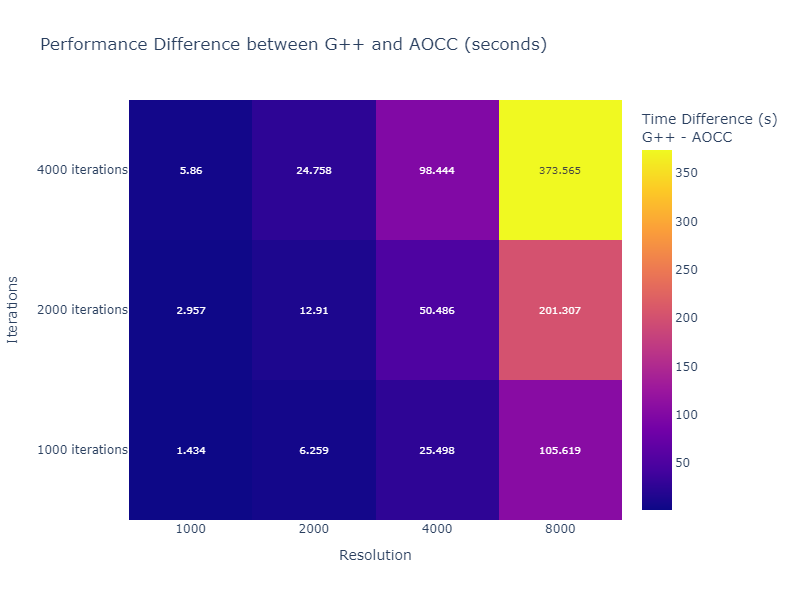
\includegraphics[width=\textwidth]{./img/mandelbrot_gcc_vs_aocc.png}
	\caption{Comparison of Execution Times for G++ and AOCC Compilers in Sequential Mandelbrot Computations.}
	\label{fig:mandelbrot_gcc_vs_aocc}
\end{figure}

\begin{figure}[H]
	\captionsetup{justification=centering, width=.8\linewidth}
	\centering
	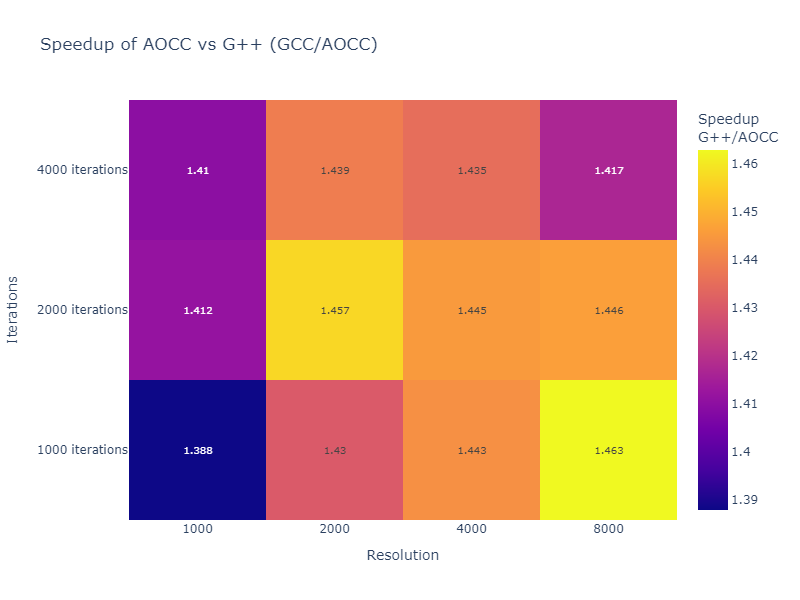
\includegraphics[width=\textwidth]{./img/mandelbrot_gcc_vs_aocc_speedup.png}
	\caption{Speedup for G++ and AOCC Compilers in Sequential Mandelbrot Computations.}
	\label{fig:mandelbrot_gcc_vs_aocc_speedup}
\end{figure}

\subsubsection{Discussion of Results}

The heatmap presented in Figure~\ref{fig:mandelbrot_aocc_seq_heatmap} illustrates the execution times for AOCC-compiled sequential Mandelbrot computations across different iterations and resolutions. As expected, both the number of iterations and the resolution significantly impact the computation time.

Higher iterations increase the computational load, while higher resolutions demand more memory and processing power to render detailed fractal images.

Figure~\ref{fig:mandelbrot_gcc_vs_aocc} compares the performance of G++ and AOCC compilers. The results indicate that while both compilers perform efficiently, AOCC exhibits a performance advantage over G++ in sequential executions up to 47\%. This difference may be attributed to the specific optimization strategies employed by each compiler and how they interact with the underlying hardware architecture. Additionally, the AOCC compiler is more optimized for AMD processors and is based on Clang. The use of additional flags such as \texttt{-mllvm} further enhances its performance by enabling advanced optimizations.

\subsubsection{Interpretation of Heatmap}

The heatmap provides a visual representation of how execution time scales with varying iterations and resolutions. Key observations include:

\begin{itemize}
	\item \textbf{Scalability:} Execution time increases linearly with the number of iterations, demonstrating predictable scalability for computationally intensive tasks.
	\item \textbf{Resolution Impact:} Higher resolutions exponentially increase execution time due to the quadratic growth in the number of points evaluated in the complex plane.
	\item \textbf{Optimization Effectiveness:} Compiler optimizations significantly reduce execution times, especially at higher iteration and resolution levels (resulting in over 370 seconds speedup), by enhancing instruction-level parallelism and cache utilization.
\end{itemize}

\subsubsection{Compiler Performance Insights}

The comparative analysis between G++ and AOCC compilers reveals nuanced differences in their optimization capabilities:

% \item GCC/G++ 13.3.0 (May 21, 2024)
% \item AOCC-compiler 5.0.0 (Clang based 17.0.6, September 24 2024)
\begin{itemize}
	\item \textbf{AOCC Advantages:} AOCC's enhanced performance, demonstrating a 38-47\% speedup over G++, can be attributed to its optimized code generation and superior exploitation of the CPU's SIMD (Single Instruction, Multiple Data) capabilities in the latest compiler version (AOCC-compiler 5.0.0, Clang-based 17.0.6, September 24, 2024).
	\item \textbf{G++ Strengths:} While AOCC outperforms G++ in this benchmark, G++ remains a robust and widely-supported compiler with extensive optimization flags and a strong community, making it versatile for various computational scenarios. There is a point that needs to be stated that G++ did not allow for certain flag naming lie -DDYNAMIC_SCHED and needed to be changed into SCHEDULE_DYNAMIC. This should be kept in mind that when trying out different compilers certain flags might not be supported.
	\item \textvf{Versioning}: This is to note that the GCC/G++ 13.3.0 compiler used in this study is a recent version, which may not fully leverage the latest hardware features of the AMD Ryzen 7 4800H CPU.
	\item \textbf{Future Considerations:} Further exploration with different optimization flags, benchmarking on diverse hardware configurations, and evaluating performance across other computational tasks could provide deeper insights into the compilers' capabilities.
\end{itemize}

\subsection{OpenMP Execution}

OpenMP was employed to exploit shared-memory parallelism in the Mandelbrot Set computations. This subsection presents the performance analysis of the OpeDifferent Thread CountsnMP implementation, focusing on execution times, speedup comparisons, scheduling strategies, and scalability with varying numbers of threads.

\subsubsection{Single-Thread Performance}

To assess the overhead introduced by OpenMP, a sequential execution was compared with an OpenMP execution utilizing a single thread. Table~\ref{tab:mandelbrot_gcc_vs_aocc_comparison} presents the execution times for AOCC-compiled sequential Mandelbrot computations across different iterations and resolutions.

Figure~\ref{fig:mandelbrot_openMP_1_thread_heatmap} illustrates the execution times for the OpenMP implementation with a single thread. Comparing Figure~\ref{fig:mandelbrot_aocc_seq_heatmap} and Figure~\ref{fig:mandelbrot_openMP_1_thread_heatmap} reveals the overhead associated with initializing and managing OpenMP parallel regions, even when only one thread is utilized.

\begin{figure}[H]
	\captionsetup{justification=centering, width=.8\linewidth}
	\centering
	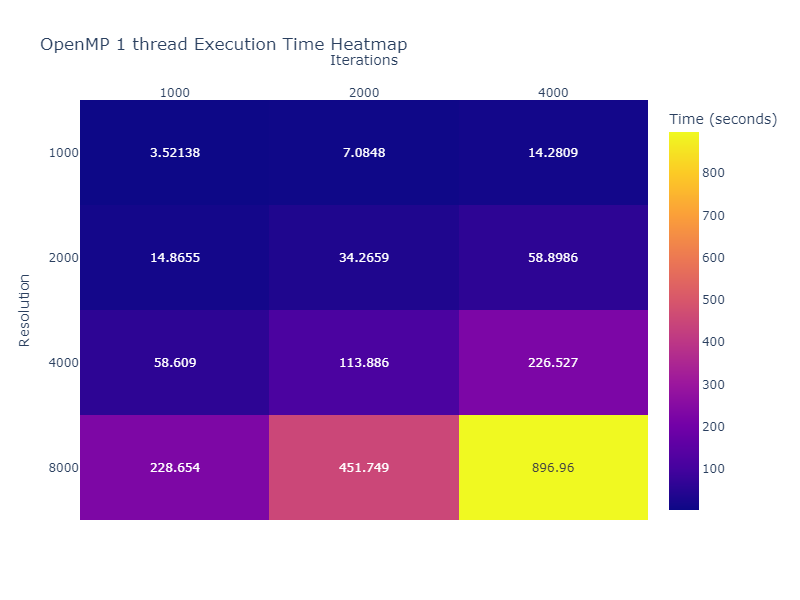
\includegraphics[width=\textwidth]{./img/mandelbrot_openmp_1_thread_heatmap.png}
	\caption{Heatmap of Execution Times for OpenMP Mandelbrot Computations with One Thread using AOCC Compiler.}
	\label{fig:mandelbrot_openMP_1_thread_heatmap}
\end{figure}

\subsubsection{Speedup Analysis with One Thread}

To quantify the overhead introduced by OpenMP, a speedup comparison between the sequential execution and the OpenMP execution with one thread was conducted. Figure~\ref{fig:mandelbrot_openMP_1_thread_speedup} highlights the speedup achieved (or lack thereof) when using a single thread in the OpenMP implementation.

\begin{figure}[H]
	\centering
	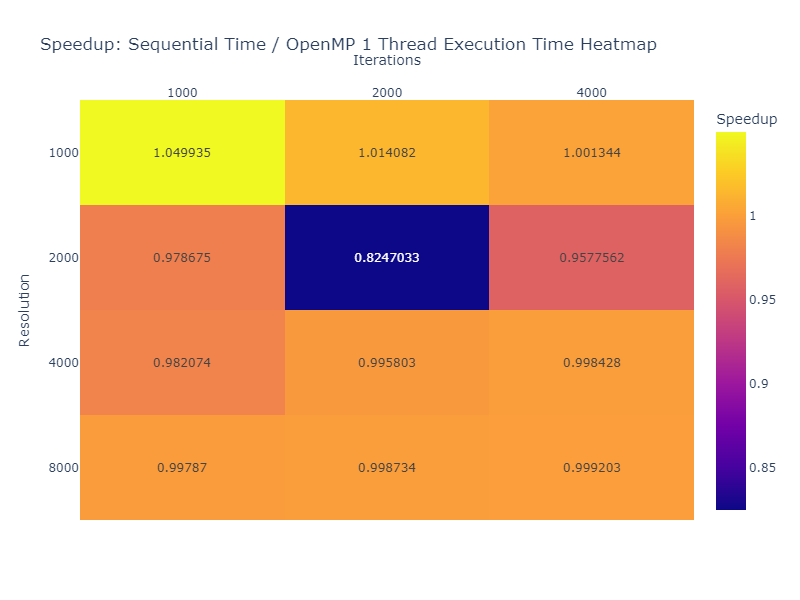
\includegraphics[width=\textwidth]{./img/mandelbrot_openmp_1_thread_speedup_heatmap.png}
	\caption{Speedup Comparison between Sequential Execution and OpenMP Execution with One Thread.}
	\label{fig:mandelbrot_openMP_1_thread_speedup}
\end{figure}

The results indicate that the OpenMP implementation with a single thread incurs a slight overhead compared to the purely sequential execution. This overhead is attributed to the overhead of managing OpenMP threads and parallel regions, which is minimal but noticeable when no actual parallelism is exploited.

\subsubsection{Impact of Scheduling Strategies}

Different OpenMP scheduling strategies can significantly influence the performance of parallel applications. Table~\ref{tab:performance_tables} showcases the execution times for various scheduling types—Dynamic, Static, Guided, and Runtime—across an increasing number of threads.

\begin{table}[H]
	\begin{adjustwidth}{-4cm}{-4cm} % Adjust margins as needed
		\centering
		\begin{subtable}[t]{0.65\textwidth}
			\centering
			\caption{2 Threads}
			\label{tab:threads_2}

			% Apply row colors starting from row 2 (after header)
			\rowcolors{2}{gray!25}{white}
			\begin{adjustbox}{width=\textwidth}
				\begin{tabular}{llcccc}
\toprule
Iterations & Resolution & DYNAMIC & GUIDED & RUNTIME & STATIC \\
\midrule
1000 & 1000 & \fcolorbox{green}{white}{2.129} & 2.138 & 2.134 & \fcolorbox{yellow}{white}{2.214} \\
1000 & 2000 & 8.627 & 8.675 & \fcolorbox{green}{white}{8.496} & \fcolorbox{yellow}{white}{8.788} \\
1000 & 4000 & \fcolorbox{yellow}{white}{35.053} & 34.831 & \fcolorbox{green}{white}{33.662} & 34.812 \\
1000 & 8000 & \fcolorbox{yellow}{white}{143.602} & 139.756 & \fcolorbox{green}{white}{133.960} & 140.192 \\
2000 & 1000 & 4.086 & 4.282 & \fcolorbox{green}{white}{4.049} & \fcolorbox{yellow}{white}{4.299} \\
2000 & 2000 & 17.076 & 17.166 & \fcolorbox{green}{white}{16.763} & \fcolorbox{yellow}{white}{17.303} \\
2000 & 4000 & 68.089 & \fcolorbox{yellow}{white}{68.381} & \fcolorbox{green}{white}{66.629} & 68.191 \\
2000 & 8000 & \fcolorbox{yellow}{white}{277.466} & 271.674 & \fcolorbox{green}{white}{264.764} & 274.310 \\
4000 & 1000 & \fcolorbox{yellow}{white}{8.533} & 8.489 & \fcolorbox{green}{white}{8.194} & 8.501 \\
4000 & 2000 & 33.572 & \fcolorbox{yellow}{white}{34.197} & \fcolorbox{green}{white}{33.531} & 33.995 \\
4000 & 4000 & 135.755 & \fcolorbox{yellow}{white}{135.841} & \fcolorbox{green}{white}{131.396} & 135.575 \\
4000 & 8000 & \fcolorbox{yellow}{white}{543.557} & 543.514 & \fcolorbox{green}{white}{531.994} & 541.809 \\
\bottomrule
\end{tabular}

			\end{adjustbox}
			% Reset row colors to default
			\rowcolors{1}{}{ }
		\end{subtable}
		\begin{subtable}[t]{0.64\textwidth}
			\centering
			\caption{4 Threads}
			\label{tab:threads_4}

			\rowcolors{2}{gray!25}{white}
			\begin{adjustbox}{width=\textwidth}
				\begin{tabular}{llcccc}
\toprule
Iterations & Resolution & DYNAMIC & GUIDED & RUNTIME & STATIC \\
\midrule
1000 & 1000 & \fcolorbox{green}{white}{1.219} & 1.226 & 1.723 & \fcolorbox{yellow}{white}{1.861} \\
1000 & 2000 & 4.941 & \fcolorbox{green}{white}{4.908} & 7.077 & \fcolorbox{yellow}{white}{7.388} \\
1000 & 4000 & 19.631 & \fcolorbox{green}{white}{19.399} & 28.512 & \fcolorbox{yellow}{white}{29.369} \\
1000 & 8000 & \fcolorbox{green}{white}{79.057} & 79.543 & 114.801 & \fcolorbox{yellow}{white}{117.315} \\
2000 & 1000 & 2.372 & \fcolorbox{green}{white}{2.337} & 3.557 & \fcolorbox{yellow}{white}{3.570} \\
2000 & 2000 & 9.481 & \fcolorbox{green}{white}{9.399} & 14.254 & \fcolorbox{yellow}{white}{14.341} \\
2000 & 4000 & \fcolorbox{green}{white}{38.274} & 38.861 & 56.409 & \fcolorbox{yellow}{white}{57.786} \\
2000 & 8000 & 154.124 & \fcolorbox{green}{white}{152.419} & 227.191 & \fcolorbox{yellow}{white}{231.310} \\
4000 & 1000 & \fcolorbox{green}{white}{4.606} & 4.683 & 6.996 & \fcolorbox{yellow}{white}{7.143} \\
4000 & 2000 & 19.105 & \fcolorbox{green}{white}{18.916} & 28.216 & \fcolorbox{yellow}{white}{29.002} \\
4000 & 4000 & \fcolorbox{green}{white}{75.252} & 77.396 & 113.111 & \fcolorbox{yellow}{white}{114.581} \\
4000 & 8000 & 303.238 & \fcolorbox{green}{white}{273.351} & 453.303 & \fcolorbox{yellow}{white}{461.844} \\
\bottomrule
\end{tabular}

			\end{adjustbox}
			\rowcolors{1}{}{ }
		\end{subtable}

		\vspace{0.2cm} % Reduced space between rows

		% Second Row: 8 Threads and 16 Threads
		\begin{subtable}[t]{0.65\textwidth}
			\centering
			\caption{8 Threads}
			\label{tab:threads_8}

			\rowcolors{2}{gray!25}{white}
			\begin{adjustbox}{width=\textwidth}
				\begin{tabular}{llcccc}
\toprule
Iterations & Resolution & DYNAMIC & GUIDED & RUNTIME & STATIC \\
\midrule
1000 & 1000 & \fcolorbox{green}{white}{0.697} & 0.703 & \fcolorbox{yellow}{white}{1.124} & 1.097 \\
1000 & 2000 & 2.718 & \fcolorbox{green}{white}{2.627} & \fcolorbox{yellow}{white}{4.707} & 4.673 \\
1000 & 4000 & 10.936 & \fcolorbox{green}{white}{10.829} & 18.697 & \fcolorbox{yellow}{white}{18.850} \\
1000 & 8000 & 43.660 & \fcolorbox{green}{white}{43.212} & 74.748 & \fcolorbox{yellow}{white}{76.018} \\
2000 & 1000 & 1.338 & \fcolorbox{green}{white}{1.321} & \fcolorbox{yellow}{white}{2.253} & 2.235 \\
2000 & 2000 & \fcolorbox{green}{white}{5.281} & 5.335 & \fcolorbox{yellow}{white}{9.339} & 9.315 \\
2000 & 4000 & 21.387 & \fcolorbox{green}{white}{21.264} & 37.005 & \fcolorbox{yellow}{white}{37.612} \\
2000 & 8000 & 85.644 & \fcolorbox{green}{white}{85.000} & 147.932 & \fcolorbox{yellow}{white}{150.229} \\
4000 & 1000 & 2.666 & \fcolorbox{green}{white}{2.591} & \fcolorbox{yellow}{white}{4.633} & 4.598 \\
4000 & 2000 & 10.551 & \fcolorbox{green}{white}{10.510} & 18.426 & \fcolorbox{yellow}{white}{18.772} \\
4000 & 4000 & 42.276 & \fcolorbox{green}{white}{42.127} & 73.802 & \fcolorbox{yellow}{white}{74.782} \\
4000 & 8000 & 169.471 & \fcolorbox{green}{white}{168.735} & 294.856 & \fcolorbox{yellow}{white}{300.303} \\
\bottomrule
\end{tabular}

			\end{adjustbox}
			\rowcolors{1}{}{ }
		\end{subtable}
		\begin{subtable}[t]{0.64\textwidth}
			\centering
			\caption{16 Threads}
			\label{tab:threads_16}

			\rowcolors{2}{gray!25}{white}
			\begin{adjustbox}{width=\textwidth}
				\begin{tabular}{llcccc}
\toprule
Iterations & Resolution & DYNAMIC & STATIC & GUIDED & RUNTIME \\
\midrule
1000 & 1000 & \fcolorbox{green}{white}{0.491} & 0.497 & \fcolorbox{yellow}{white}{0.736} & 0.729 \\
1000 & 2000 & \fcolorbox{green}{white}{1.762} & 1.764 & 2.667 & \fcolorbox{yellow}{white}{2.721} \\
1000 & 4000 & 6.854 & \fcolorbox{green}{white}{6.818} & 10.759 & \fcolorbox{yellow}{white}{10.955} \\
1000 & 8000 & \fcolorbox{green}{white}{26.886} & 27.053 & 43.284 & \fcolorbox{yellow}{white}{44.112} \\
2000 & 1000 & 0.911 & \fcolorbox{green}{white}{0.887} & 1.289 & \fcolorbox{yellow}{white}{1.325} \\
2000 & 2000 & \fcolorbox{green}{white}{3.356} & 3.405 & \fcolorbox{yellow}{white}{5.469} & 5.428 \\
2000 & 4000 & \fcolorbox{green}{white}{13.206} & 13.357 & \fcolorbox{yellow}{white}{21.610} & 21.564 \\
2000 & 8000 & \fcolorbox{green}{white}{52.668} & 54.010 & 86.582 & \fcolorbox{yellow}{white}{86.656} \\
4000 & 1000 & \fcolorbox{green}{white}{1.691} & 1.728 & 2.687 & \fcolorbox{yellow}{white}{2.733} \\
4000 & 2000 & \fcolorbox{green}{white}{6.574} & 6.652 & \fcolorbox{yellow}{white}{10.834} & 10.755 \\
4000 & 4000 & \fcolorbox{green}{white}{26.109} & 26.223 & 42.965 & \fcolorbox{yellow}{white}{43.315} \\
4000 & 8000 & \fcolorbox{green}{white}{105.083} & 105.125 & 172.743 & \fcolorbox{yellow}{white}{172.940} \\
\bottomrule
\end{tabular}

			\end{adjustbox}
			\rowcolors{1}{}{ }
		\end{subtable}

		\vspace{0.2cm}
		\noindent \textbf{Legend:} \fcolorbox{yellow}{white}{\rule{0pt}{4pt}\rule{4pt}{0pt}} = Highest Execution Time, \fcolorbox{green}{white}{\rule{0pt}{4pt}\rule{4pt}{0pt}} = Lowest Execution Time
		\captionsetup{justification=centering, width=.8\linewidth}
		\caption{Mandelbrot Program Performance Across Different Thread Counts}
		\label{tab:performance_tables}
	\end{adjustwidth}
\end{table}

\begin{figure}[H]
	\centering
	\captionsetup{justification=centering, width=.8\linewidth}
	\includegraphics[width=\textwidth]{./img/mandelbrot_openMP_scheduling_types_heatmap_speedup.png}
	\caption{Execution Times for OpenMP Mandelbrot Computations with Various Scheduling Types and Increasing Threads.}
	\label{fig:mandelbrot_openMP_scheduling_types_heatmap_speedup}
\end{figure}

Dynamic scheduling demonstrates superior performance over static and runtime approaches across thread configurations. While Guided scheduling shows comparable efficiency and performs marginally better with 4 threads, Dynamic scheduling maintains better performance scaling at 16 threads, indicating better adaptability to increased parallelism.

\subsubsection{Scalability and Speedup with Multiple Threads}

To evaluate the scalability of the OpenMP implementation, speedup was measured as the number of threads increased from 2 to 16. Figure~\ref{fig:mandelbrot_openMP_best_speedup_vs_threads} presents the speedup achieved for various configurations of resolutions and iterations. Additionally, Figure~\ref{fig:mandelbrot_openMP_best_speedup_vs_threads_heatmap} provides a heatmap representation for easier data interpretation, while Figure~\ref{fig:mandelbrot_openMP_best_speedup_vs_threads_bar} offers a bar plot highlighting the best speedup scenarios with a diamond icon.

\begin{figure}[H]
	\centering
	\captionsetup{justification=centering, width=.8\linewidth}
	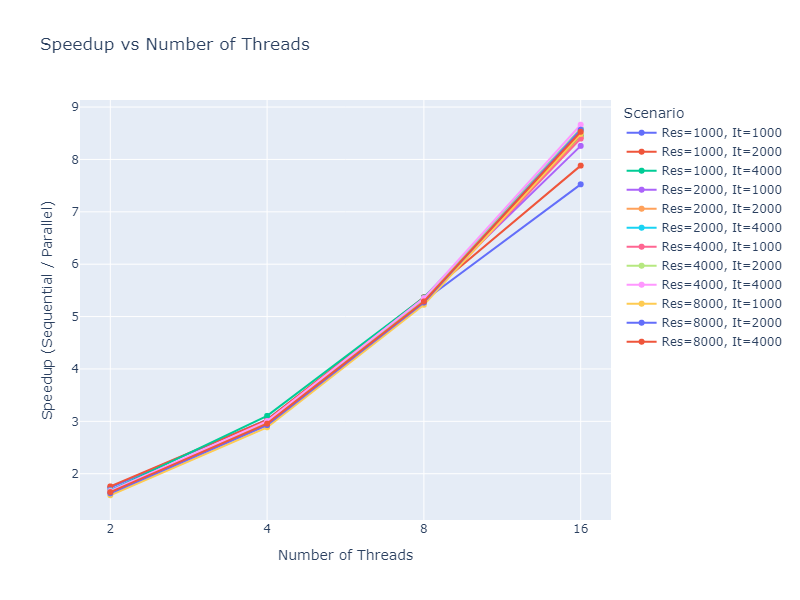
\includegraphics[width=\textwidth]{./img/mandelbrot_openmp_best_speedup_vs_threads.png}
	\caption{Speedup of OpenMP Mandelbrot Computations with Increasing Number of Threads for Various Resolutions and Iterations for Dynamic Scheduling.}
	\label{fig:mandelbrot_openMP_best_speedup_vs_threads}
\end{figure}

\begin{figure}[H]
	\centering
	\captionsetup{justification=centering, width=.8\linewidth}
	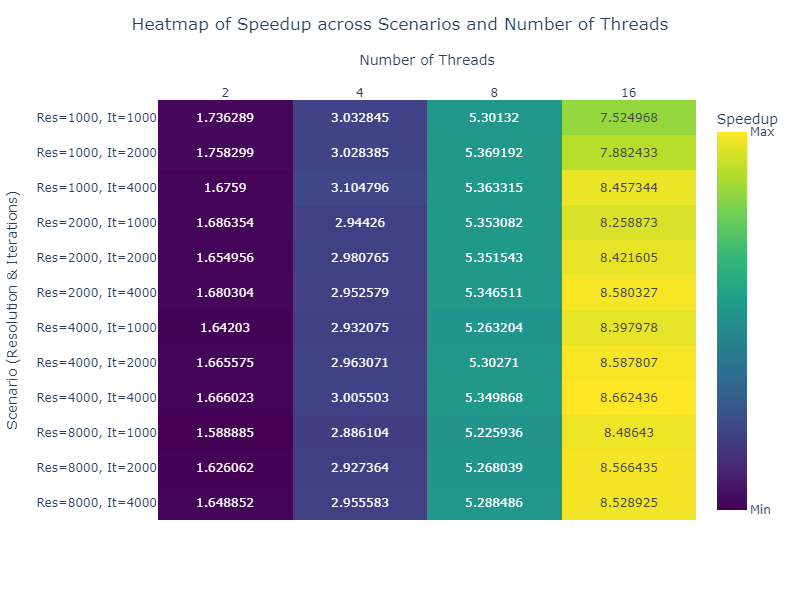
\includegraphics[width=\textwidth]{./img/mandelbrot_openmp_best_speedup_vs_threads_heatmap.png}
	\caption{Heatmap of Speedup for OpenMP Mandelbrot Computations with Varying Threads, Resolutions, and Iterations for Dynamic Scheduling.}
	\label{fig:mandelbrot_openMP_best_speedup_vs_threads_heatmap}
\end{figure}

\begin{figure}[H]
	\centering
	\captionsetup{justification=centering, width=.8\linewidth}
	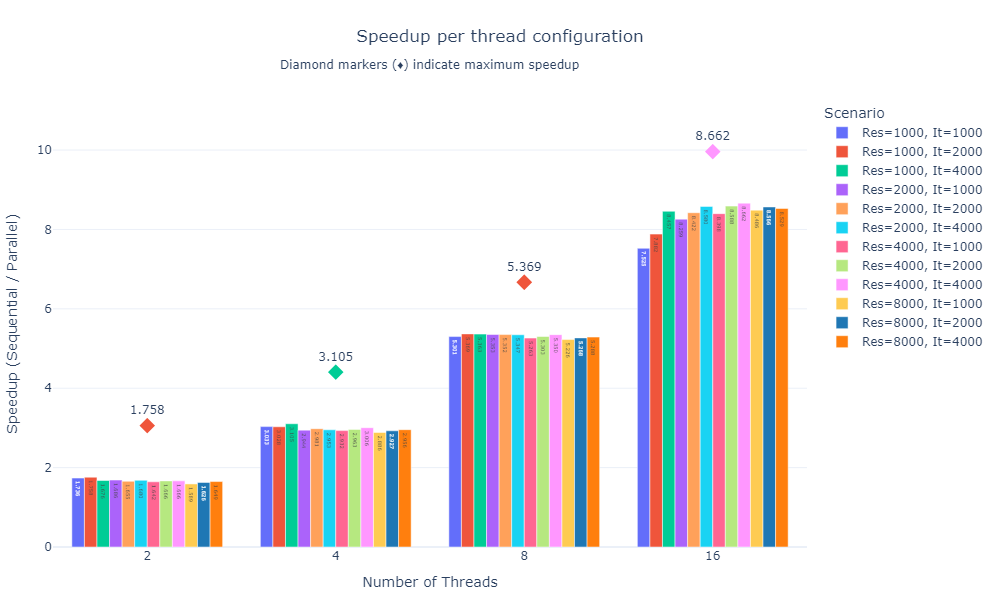
\includegraphics[width=\textwidth]{./img/mandelbrot_openmp_best_speedup_vs_threads_bar.png}
	\caption{Bar Plot of Speedup for OpenMP Mandelbrot Computations with Highlighted Best Scenarios for Dynamic Scheduling.}
	\label{fig:mandelbrot_openMP_best_speedup_vs_threads_bar}
\end{figure}

The heatmap in Figure~\ref{fig:mandelbrot_openMP_best_speedup_vs_threads_heatmap} and the corresponding bar plot in Figure~\ref{fig:mandelbrot_openMP_best_speedup_vs_threads_bar} illustrate that the OpenMP implementation scales efficiently with the number of threads, achieving significant speedups up to 16 threads. The best speedup scenarios are highlighted, demonstrating optimal performance for higher resolutions and iterations where parallelism is most beneficial.

\subsubsection{Overall OpenMP Performance}

Overall, the OpenMP implementation demonstrates substantial performance improvements over the sequential execution, particularly when utilizing multiple threads and Dynamic scheduling. The ability to effectively distribute the computational workload across multiple cores leads to reduced execution times and enhanced scalability.

\subsubsection{Summary of OpenMP Results}

The OpenMP benchmarks reveal the following key insights:

\begin{itemize}
	\item \textbf{Overhead Assessment:} OpenMP introduces minimal overhead when using a single thread, ensuring that performance remains comparable to sequential execution. It is possible that due to the lightweight nature of the OpenMP constructs, the overhead is negligible and not included in binary code by the compiler.
	\item \textbf{Scheduling Strategy Impact:} Dynamic scheduling outperforms other scheduling types, providing better load balancing and higher speedups as thread counts increase.
	\item \textbf{Scalability:} The OpenMP implementation scales effectively with the number of threads, achieving near-linear speedup for moderate thread counts and complex computational tasks.
	\item \textbf{Optimal Configurations:} Higher resolutions and iteration counts benefit more from parallelization, highlighting the effectiveness of OpenMP in handling computationally intensive scenarios.
\end{itemize}

\subsection{CUDA GPU Acceleration}

To leverage the parallel processing capabilities of modern GPUs, a CUDA implementation of the Mandelbrot Set computation was developed. This implementation was specifically optimized to utilize the NVIDIA GeForce RTX 2060 GPU, which features 1920 CUDA cores and supports high levels of parallelism. The CUDA version was designed to handle high-resolution fractal images with a substantial number of iterations, thereby demonstrating significant speedup compared to the sequential execution.

\subsubsection{Speedup Analysis}

The performance of the CUDA implementation was evaluated by comparing its execution time against the sequential baseline. The benchmark was conducted using a resolution of 8000 pixels and 4000 iterations, which are computationally intensive parameters that push the GPU to its limits. The speedup achieved by the CUDA implementation was measured across various thread block sizes, specifically using 4, 16, 64, 256, and 1024 CUDA threads. The results are summarized in Table~\ref{tab:cuda_performance} and visualized in Figure~\ref{fig:mandelbrot_cuda_speedup_vs_threads_amdahl}.


\begin{table}[H]
	\captionsetup{justification=centering, width=.8\linewidth}
	\centering
	\caption{CUDA Mandelbrot Program Performance}
	\label{tab:cuda_performance}

	\rowcolors{2}{gray!25}{white} % Apply striped rows starting from the second row
	\begin{adjustbox}{max width=\textwidth}
		\begin{tabular}{llccccc}
	\toprule
	Iterations & Resolution & 4 Threads & 16 Threads & 64 Threads & 256 Threads & 1024 Threads \\
	\midrule
	1000       & 1000       & 4.242     & 1.295      & 0.678      & 0.716       & 0.673        \\
	1000       & 2000       & 16.426    & 4.719      & 2.268      & 2.339       & 2.192        \\
	1000       & 4000       & 66.178    & 18.845     & 9.048      & 8.846       & 8.901        \\
	1000       & 8000       & 284.385   & 71.540     & 35.899     & 39.020      & 34.246       \\
	2000       & 1000       & 8.062     & 2.362      & 1.110      & 1.162       & 1.114        \\
	2000       & 2000       & 32.491    & 9.622      & 4.565      & 4.569       & 4.410        \\
	2000       & 4000       & 139.467   & 36.761     & 17.477     & 17.499      & 16.810       \\
	2000       & 8000       & 532.693   & 137.950    & 69.975     & 74.731      & 66.489       \\
	4000       & 1000       & 15.935    & 4.604      & 2.210      & 2.363       & 2.200        \\
	4000       & 2000       & 64.509    & 18.700     & 8.752      & 9.032       & 8.422        \\
	4000       & 4000       & 290.635   & 69.233     & 34.590     & 36.787      & 33.306       \\
	4000       & 8000       & 1067.240  & 273.820    & 138.460    & 132.968     & 131.760      \\
	\bottomrule
\end{tabular}

	\end{adjustbox}
	\rowcolors{1}{}{ } % Reset row colors
\end{table}


The plot in Figure~\ref{fig:mandelbrot_cuda_speedup_vs_threads_amdahl} illustrates the speedup achieved by the CUDA implementation as the number of CUDA threads increases. Notably, the speedup scales significantly with the number of threads, demonstrating the GPU's ability to handle parallel tasks efficiently. As the thread count increases, the execution time decreases, showcasing the effectiveness of CUDA's parallel architecture in accelerating computationally demanding tasks like Mandelbrot Set computations.

\subsubsection{CUDA Kernel Implementation}

The core computation in the CUDA implementation is encapsulated within two kernel functions: \texttt{dev\_Mandelbrot\_kernel} and \texttt{mandelbrotKernel}. The \texttt{dev\_Mandelbrot\_kernel} function performs the iterative calculation to determine the membership of each point in the Mandelbrot Set, while the \texttt{mandelbrotKernel} function manages the parallel execution across the GPU threads.

\begin{lstlisting}[language=C++, caption={CUDA Kernel Functions for Mandelbrot Set Computation}, label={lst:mandelbrot_cuda}]
__device__ int dev_Mandelbrot_kernel(int collumn, int row,
                                     double step, int minX,
                                     int minY, int iterations)
{
    int count = 0;

    cuDoubleComplex c = make_cuDoubleComplex(minX + collumn * step,
                                            minY + row * step);
    cuDoubleComplex z = make_cuDoubleComplex(0, 0);
    while (cuCabs(z) < 2.0 && count < iterations)
    {
        z = cuCadd(cuCmul(z, z), c);
        count++;
    }

    return (count < iterations) ? count : 0;
}

__global__ void mandelbrotKernel(int *image, double step, int minX,
                                 int minY, int iterations,
                                 int WIDTH, int HEIGHT)
{
    // Idiomatic CUDA loop
    int col = blockIdx.x * blockDim.x + threadIdx.x;
    int row = blockIdx.y * blockDim.y + threadIdx.y;
    if (col >= WIDTH || row >= HEIGHT)
        return;

    int index = row * WIDTH + col;
    image[index] = dev_Mandelbrot_kernel(col, row, step, minX, minY,
                                         iterations);
}
\end{lstlisting}

\subsubsection{Performance Insights}

The CUDA implementation demonstrates substantial speedup, especially when the GPU is fully utilized with a high number of threads. According to Amdahl's Law, the theoretical maximum speedup is limited by the serial portion of the computation. However, in this scenario, the parallel portion dominates, allowing the CUDA implementation to achieve near-linear speedup as the number of threads increases.

\begin{figure}[H]
	\captionsetup{justification=centering, width=.8\linewidth}
	\centering
	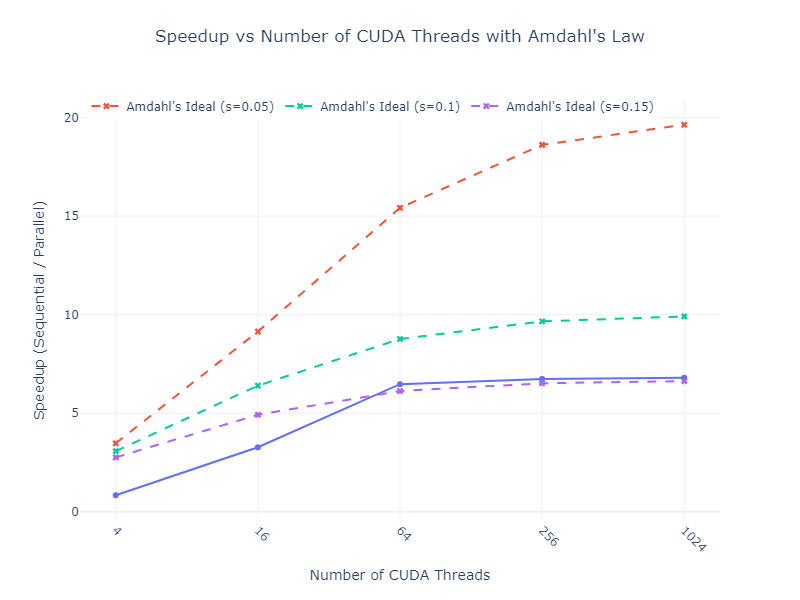
\includegraphics[width=\textwidth]{./img/mandelbrot_cuda_speedup_vs_threads_amdahl.png}
	\caption{Speedup of CUDA Mandelbrot Computations Compared to Sequential Execution for Resolution 8000 and Iterations 4000.}
	\label{fig:mandelbrot_cuda_speedup_vs_threads_amdahl}
\end{figure}

The plot in Figure~\ref{fig:mandelbrot_cuda_speedup_vs_threads_amdahl} showcases the speedup achieved by the CUDA implementation relative to the sequential execution. As the number of CUDA threads increases from 4 to 1024, the speedup grows proportionally, highlighting the GPU's capacity to handle extensive parallel workloads effectively.

\subsubsection{Conclusion of CUDA Results}

The CUDA implementation of the Mandelbrot Set computation effectively harnesses the parallel processing power of the NVIDIA GeForce RTX 2060 GPU, achieving substantial speedup compared to sequential execution. By scaling the number of CUDA threads, the implementation demonstrates excellent scalability and efficiency, making it a powerful tool for generating high-resolution fractal images with a large number of iterations. The ability to push the GPU to its computational limits results in impressive performance gains, validating the efficacy of GPU acceleration in high-performance computing applications.

\subsubsection{Summary of CUDA Results}

The CUDA benchmarks reveal the following key insights:

\begin{itemize}
	\item \textbf{Scalability:} The CUDA implementation scales effectively with the number of threads, achieving significant speedup as the thread count increases.
	\item \textbf{Performance Gains:} Pushing the GPU to its limits with high thread counts results in much larger speedup compared to sequential execution.
	\item \textbf{Optimization Potential:} Further optimizations, such as memory management and kernel tuning, could enhance performance even more.
	\item \textbf{Parallel Efficiency:} The highly parallel nature of the Mandelbrot computation aligns well with the GPU architecture, maximizing computational throughput.
\end{itemize}

\subsection{MPI Distributed Computing}

The Message Passing Interface (MPI) was utilized to implement distributed-memory parallelism for the Mandelbrot Set computations. MPI enables the distribution of computational tasks across multiple nodes in a cluster, facilitating the handling of large-scale problems by leveraging the combined processing power and memory of several interconnected machines. This subsection discusses the implementation challenges, performance metrics, and scalability analysis of the MPI-based Mandelbrot computations.

\subsubsection{Implementation Overview}

The MPI implementation was developed using the \texttt{mpiicpc} compiler, which supports parallel execution across multiple hosts. The core strategy involved distributing the Mandelbrot computation tasks among various MPI processes, each potentially utilizing multiple threads via OpenMP for intra-process parallelism. The Makefile targets \texttt{compile-mpi} and \texttt{run-mpi} were employed to compile and execute the MPI-based Mandelbrot program. The benchmarking focused on varying the number of MPI processes and observing the corresponding speedup relative to the sequential execution.

\subsubsection{Issue with Thread Management}

During the implementation, an unintended interaction between MPI processes and OpenMP threads arose. Specifically, the use of \texttt{omp\_get\_max\_threads()} within the MPI code led to each MPI process spawning all available threads on the host machine. For instance, on a machine with a processor supporting 16 threads, running the program with \texttt{-np 4} (4 MPI processes) resulted in each process attempting to utilize 16 threads, culminating in a total of 64 threads per machine. This behavior was contrary to the initial intention of allocating a fixed number of threads per process (e.g., 4 threads per process).

As the number of MPI processes increased, the number of threads per process inadvertently decreased, leading to suboptimal utilization of the CPU cores and diminishing the expected speedup. This misconfiguration impeded the scalability of the MPI implementation, particularly noticeable when scaling beyond a single host.

\subsubsection{Speedup Analysis}

The performance of the MPI implementation was evaluated by measuring the speedup achieved relative to the sequential execution as the number of MPI processes varied. Two primary plots were generated to illustrate the speedup behavior:

\begin{itemize}
	\item \textbf{Speedup vs. Number of Processes:} Figure~\ref{fig:mandelbrot_mpi_speedup_vs_processes_bar} showcases the speedup achieved across a range of MPI processes from 4 to 256 across 4 hosts.
	\item \textbf{Normalized Speedup:} \texttt{mandelbrot\_mpi\_speedup\_vs\_processes.png} presents the speedup for 64, 128, and 256 MPI processes, each utilizing 4 threads.
\end{itemize}

\begin{table}[H]
	\centering
	\captionsetup{justification=centering, width=.8\linewidth}
	\begin{tabular}{lrrrr}
\toprule
Machines & Processes & Threads & Time (seconds) & Speedup \\
\midrule
1 & 4 & 64 & 84.870 & 10.560 \\
1 & 8 & 32 & 99.540 & 9.004 \\
1 & 16 & 16 & 104.066 & 8.612 \\
1 & 32 & 8 & 106.892 & 8.385 \\
1 & 64 & 4 & 104.814 & 8.551 \\
2 & 8 & 64 & 99.451 & 9.012 \\
2 & 16 & 32 & 104.229 & 8.599 \\
2 & 32 & 16 & 106.746 & 8.396 \\
2 & 64 & 8 & 104.571 & 8.571 \\
2 & 128 & 8 & 61.255 & 14.631 \\
4 & 16 & 64 & 104.015 & 8.616 \\
4 & 32 & 32 & 106.633 & 8.405 \\
4 & 64 & 16 & 104.828 & 8.550 \\
4 & 128 & 16 & 61.257 & 14.631 \\
4 & 256 & 16 & 34.710 & 25.821 \\
\bottomrule
\end{tabular}

	\caption{Speedup of MPI Mandelbrot Computations with Varying Number of Processes Across Multiple Hosts.}
	\label{tab:mandelbrot_mpi_speedup_vs_processes}
\end{table}

\begin{figure}[H]
	\centering

	\captionsetup{justification=centering, width=.8\linewidth}
	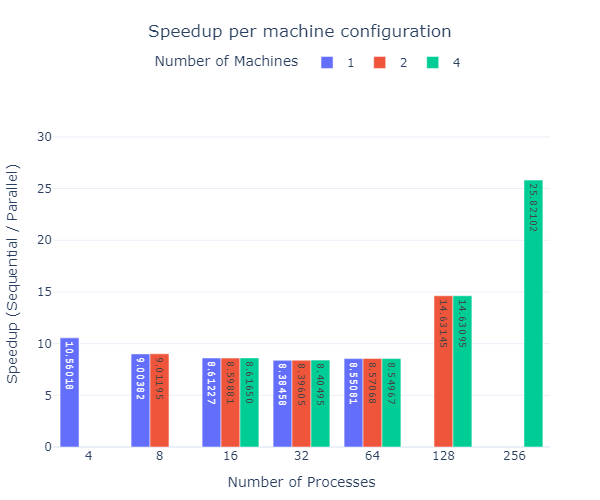
\includegraphics[width=\textwidth]{./img/mandelbrot_mpi_speedup_vs_processes_bar.png}
	\caption{Speedup of MPI Mandelbrot Computations with Varying Number of Processes Across Multiple Hosts.}
	\label{fig:mandelbrot_mpi_speedup_vs_processes_bar}
\end{figure}
\begin{figure}[H]
	\centering
	\captionsetup{justification=centering, width=.8\linewidth}
	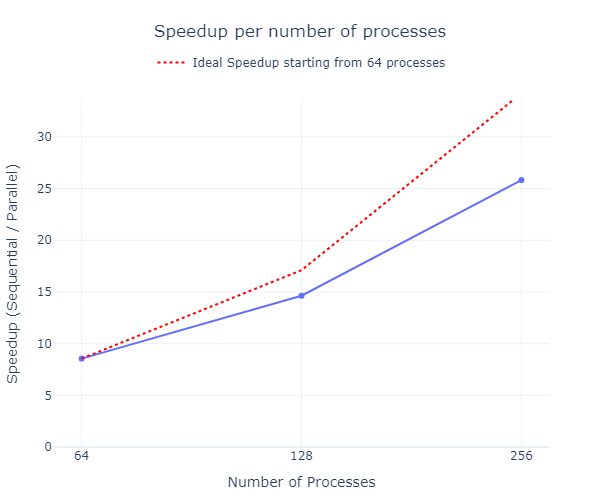
\includegraphics[width=\textwidth]{./img/mandelbrot_mpi_speedup_vs_processes.png}
	\caption{Speedup of MPI Mandelbrot Computations with 64, 128, and 256 Processes Utilizing 4 Threads Each.}
	\label{fig:mandelbrot_mpi_speedup_vs_processes}
\end{figure}


\subsubsection{Code Snippet Highlighting the Issue}

The following code snippet from the MPI implementation demonstrates the unintended thread allocation due to the use of \texttt{omp\_get\_max\_threads()}:

\begin{lstlisting}[language=C++, caption={MPI Mandelbrot Kernel Launch with Thread Mismanagement}, label={lst:mandelbrot_mpi_code}]
	// Setting max threads per node
	int threads_used = omp_get_max_threads();
	omp_set_num_threads(threads_used);

	auto start_time = chrono::steady_clock::now();

#pragma omp parallel for schedule(dynamic) default(none)           \
	firstprivate(sub_image, ITERATIONS) shared(WIDTH, STEP)
	for (int pos = start_index; pos < end_index; pos++)
	{
		const int row = pos / WIDTH;
		const int col = pos % WIDTH;
		const complex<double> c(col * STEP + MIN_X,
								row * STEP + MIN_Y);

		int iter = 1;
		complex<double> z(0, 0);
		for (; iter <= ITERATIONS; iter++)
		{
			z = (z * z) + c;

			// If the magnitude exceeds 2, the point is not in the
			// Mandelbrot set if (abs(z) >= 2)
			if (((z.real() * z.real()) + (z.imag() * z.imag())) >=
				4)
			{
				sub_image[pos - start_index] = iter;
				break;
			}
		}
	}

	// Gather results from all processes to the root process
	err =
		MPI_Gather(sub_image, pixels_per_process, MPI_INT, image,
				   pixels_per_process, MPI_INT, 0, MPI_COMM_WORLD);
	checkMPIError(err, "MPI_Gather failed.");
\end{lstlisting}

The use of \texttt{omp\_get\_max\_threads()} without proper thread locking for certain number resulted in each MPI process attempting to utilize the maximum number of threads available on the host. This leads to subsitition of processes for threads.

This results in clear openMPI overhead, as the number of threads per process decreases as the number of processes increases, leading to inefficient parallel execution and diminished returns on additional processes. This overhead of processes is visible on the Figure~\ref{fig:mandelbrot_mpi_speedup_vs_processes_bar} where going from 4 processes to 64 is is a regression of speedup because processes are put in place instead of threads.


\subsubsection{Lessons Learned and Future Improvements}

The performance issues encountered with the MPI implementation highlight the necessity of meticulous thread and process management in hybrid parallel computing environments. To address the observed challenges and enhance scalability, the following improvements are proposed:

\begin{itemize}
	\item \textbf{Resource Allocation Strategy:} Develop a resource allocation strategy that balances the number of MPI processes and OpenMP threads based on the underlying hardware capabilities, ensuring optimal utilization without overloading CPU cores.
	\item \textbf{Hybrid Parallelism Optimization:} Explore hybrid parallelism techniques that effectively combine MPI and OpenMP, potentially leveraging MPI process pinning and affinity settings to enhance cache utilization and reduce communication overhead.
	\item \textbf{Dynamic Load Balancing:} Investigate dynamic load balancing mechanisms to distribute computational tasks more evenly across MPI processes and threads, mitigating the impact of uneven workload distribution.
\end{itemize}

Implementing these strategies will enable more efficient scaling of the MPI implementation, unlocking the full potential of the HPC cluster for Mandelbrot Set computations and other parallel applications.

\subsubsection{Conclusion of MPI Results}

By addressing the thread management issues and adopting a more disciplined approach to resource allocation, future implementations can achieve more significant speedup and better scalability. The insights gained from this benchmarking exercise emphasize the critical interplay between MPI processes and OpenMP threads in hybrid parallel computing environments, guiding the optimization of parallel applications for maximum performance.

\subsubsection{Summary of MPI Results}

The MPI benchmarks revealed the following key insights:

\begin{itemize}
	\item \textbf{Scalability Constraints:} Due to misconfiguration of MPI processing, the MPI implementation did not achieve the expected linear speedup. When increasing the number of processes on a single host the threads were converted into processes resulting in performance decrease.
	\item \textbf{Optimization Necessity:} Effective thread and process management is essential to harness the full potential of distributed-memory parallelism in MPI applications.
	\item \textbf{Future Directions:} Implementing controlled thread allocation and optimizing hybrid MPI/OpenMP configurations can significantly enhance scalability and performance.
\end{itemize}

These findings underscore the importance of careful parallelism strategy design in MPI implementations, especially when integrating with multi-threaded approaches like OpenMP. Proper synchronization and resource management are pivotal in achieving efficient and scalable parallel computations in HPC environments.



\end{document}